\documentclass[hyperref]{article}
%MS%%%%%%%%%%%%%%%%%%%% Article Format %%%%%%%%%%%%%%%%%
%+++++++++++++++++++++ Usepackage +++++++++++++++%%
\usepackage{graphicx} %% Package for Figure
\usepackage{float} %% Package for Float
\usepackage{amssymb}
\usepackage{amsmath}
\usepackage{mathtools}
\usepackage{multirow}
\usepackage{booktabs}
\usepackage{listings}
\usepackage{graphicx}
\usepackage[toc,page]{appendix}
\usepackage[thmmarks]{ntheorem} %% If amsmath is applied, then amsma is necessary
\usepackage{bm} %% Bold Mathematical Symbols
\usepackage[colorlinks,linkcolor=cyan,citecolor=cyan]{hyperref}
\usepackage{extarrows}
\usepackage[hang,flushmargin]{footmisc} %% Let the footnote not indentation
\usepackage[square,comma,sort&compress,numbers]{natbib} %% Sort of References
\usepackage[font=footnotesize,skip=0pt,textfont=rm,labelfont=rm]{caption,subcaption}
%% Format of Caption for Tab. and Fig.
\usepackage{booktabs} %% tables with three lines
\usepackage{tocloft}
%+++++++++++++++ Proof etc. +++++++++++++++++++++++++%%
{%% Environment of Proof
    \theoremstyle{nonumberplain}
    \theoremheaderfont{\bfseries}
    \theorembodyfont{\normalfont}
    \theoremsymbol{\mbox{$\Box$}}
    \newtheorem{proof}{Proof}
}

\usepackage{theorem}
\newtheorem{theorem}{Theorem}[section]
\newtheorem{lemma}{Lemma}[section]
\newtheorem{definition}{Definition}[section]
\newtheorem{assumption}{Assumption}[section]
\newtheorem{example}{Example}[section]
\newtheorem{corollary}{Corollary}[section]
{%% Environment of Remark
    \theoremheaderfont{\bfseries}
    \theorembodyfont{\normalfont}
    \newtheorem{remark}{Remark}[section]
}
%\numberwithin{equation}{section} %% Number of Equation
%++++++++++++++++++++++++++++++++ Page format ++++++++++++++++++++++++++%%
\graphicspath{{figure/}}                                 %% Path of Figures
\usepackage[a4paper]{geometry}                           %% Paper size
\geometry{left=2.5cm,right=2.5cm,top=2.5cm,bottom=2.5cm} %% Margin
\linespread{1.2}                                         %% Line Spread
%MS%%%%%%%%%%%%%%%%%%%%%%%%%%%% End Format %%%%%%%%%%%%%%%%%%%%%%%%%%%%%%%%%%

%MS%%%%%%%%%%%%%%%%%%%%%%%%%%%%%%%%%%%%%%%%%%%
%MS                                         %%
%MS        The Main Body begins here        %%
%MS                                         %%
%MS%%%%%%%%%%%%%%%%%%%%%%%%%%%%%%%%%%%%%%%%%%%

%MS++++++++++++++++++++++++++++++ Title +++++++++++++++++++
\begin{document}
\title{\bf CIFAR-10 Classification Problem}
%\date{}
\author{\sffamily \\ Zhilin Fan\\
    {\sffamily Professor: John Cunningham}\\
    {\sffamily GR5242 Advanced Machine Learning}}
\renewcommand{\thefootnote}{\fnsymbol{footnote}}
%\footnotetext[1]{Corresponding author. }
\maketitle

%MS+++++++++++++++++++++ Abstract +++++++++++++++++++++++++
\abstract
In this project, we built up a Convolutional Neural Network(CNN) to solve the classification problem on CIFAR-10 datasets, which consists of $60000$ $32\times32$ colour images in $10$ classes, with $6000$ images per class. And there are $50000$ training images and 10000 test images.
We began with a simple CNN model but met with a serious overfitting problem. The test accuracy was between $50\%-55\%$ while the training loss was about $0.2$ and training accuracy was about $90\%$. We tried several ways, including adding more layers, adding dropout layer, changing the activation function of the layer, but these did not make big difference. Finally, we used the following strategies: \\
1. preprocess the image data(crop image from $32\times32\times3$ to $28\times28\times3$ and add some noise in the training step \\
2. add weight decay in two fully-connected layers

Finally, we improved the performance and the accuracy was about $67\%$.

In addition, we recomputed the bottleneck and retrained the last layer of Inception-V3 model. The final test accuracy was about $ 81.5\%$.

\newpage
\tableofcontents
\newpage

%MS++++++++++++++++++++++++++++++ Main body ++++++++++++++++++++
\section{Introduction}
CIFAR-10 is a really important image classification dataset for data scientists and machine learning researchers. In the past few decades a large number of projects are finished based on CIFAR-10. In this project we are going to create our deep learning classifier for CIFAR-10 with the highest accuracy.

\section{CNN model}
In this section, we implemented a 9-layer Convolutional Neural Network to solve the CIFAR-10 classification problem. The construction of this network is as following: \\
1. a convolutional layer: filter size $[3,5,5,32]$, Relu activated \\
2. a max-pooling layer: kernel size $[2,2]$ and stride $2$ \\
3. a convolutional layer: filter size $[32,5,5,64]$, Relu activated \\
4. a max-pooling layer: kernel size $[2,2]$ and stride $2$ \\
5. a convolutional layer: filter size $[64,5,5,64]$, Relu activated \\
6. a convolutional layer: filter size $[64,3,3,32]$, Relu activated \\
7. a max-pooling layer: kernel size $[3,3]$ and stride $2$ \\
8. a fully-connected layer: filter size $[3*3*32,384]$, Relu activated, standard deviation=$0.04$, weight decay=$0.001$, biases=$0.1$ \\
9. a fully-connected layer: filter size [384,192], Relu activated, standard deviation=$0.04$, weight decay=$0.01$, biases=$0.1$ \\

The following graph shows the structure of this model: \\
\begin{figure}[htbp]
\centering
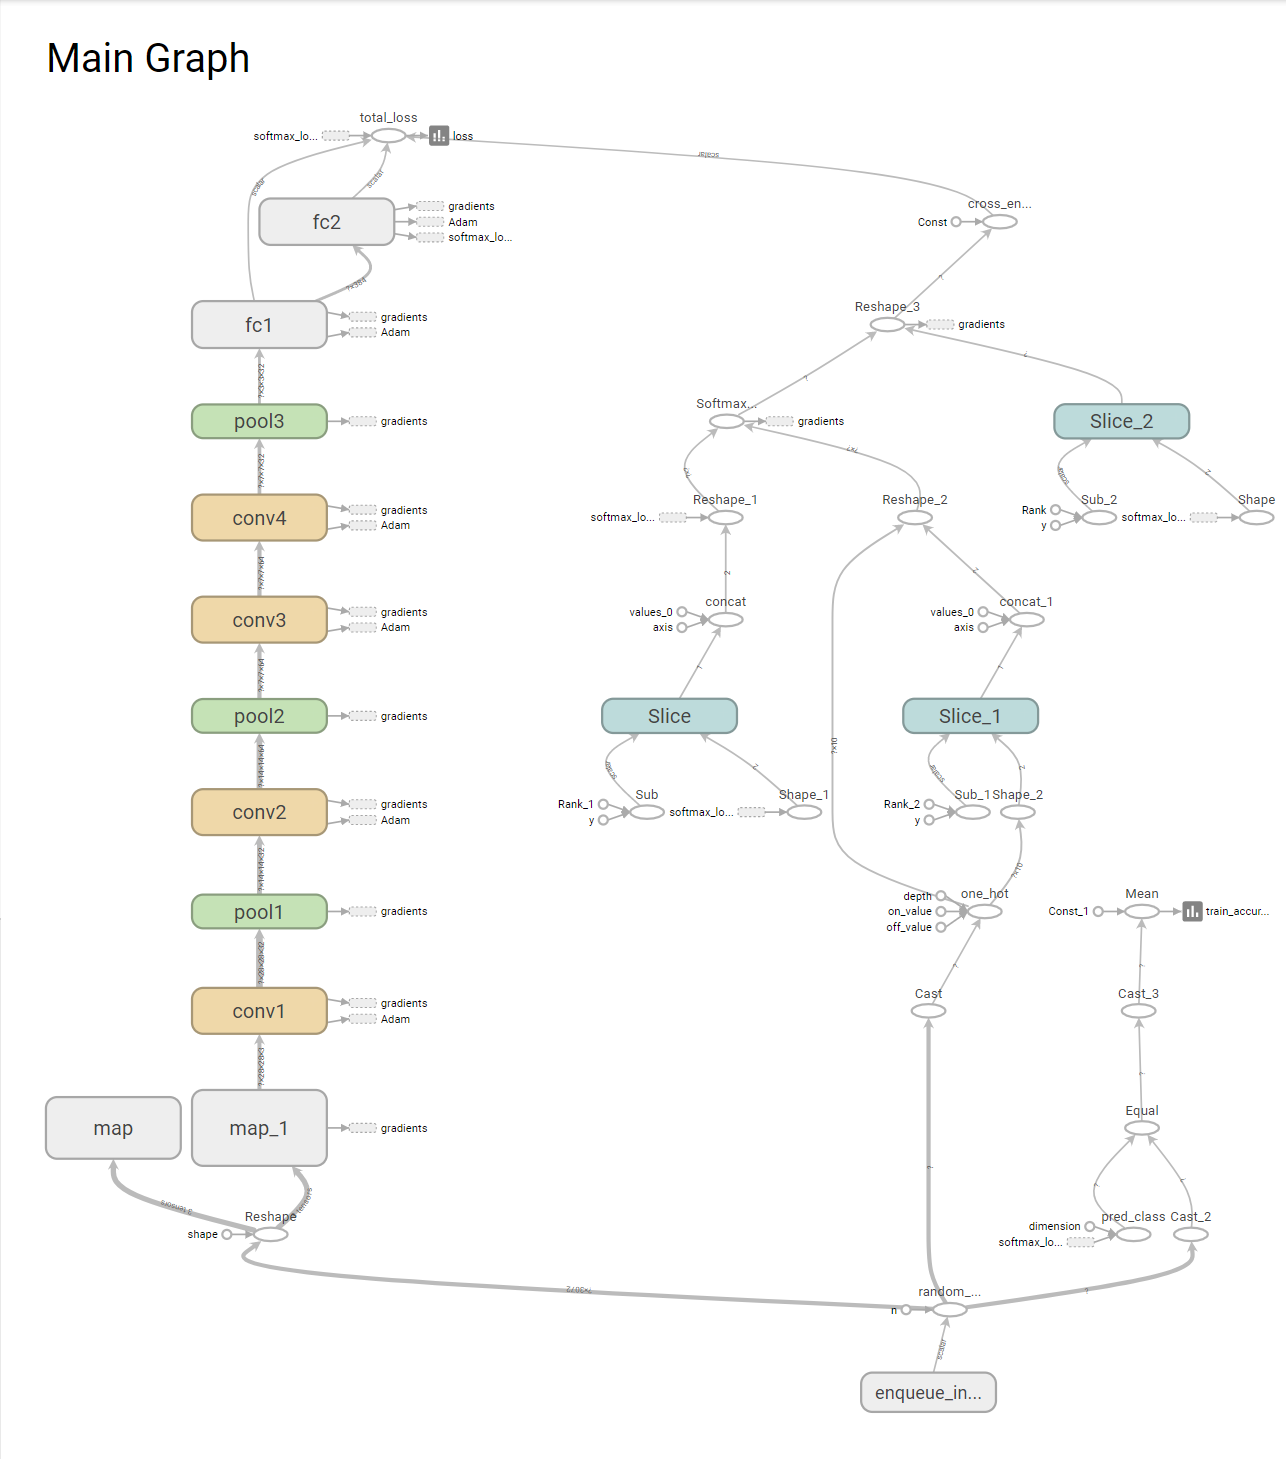
\includegraphics[height=480pt]{main_graph.png}
\caption{CNN model}
\label{main}
\end{figure}

At the beginning, we trained the network without any preprocessing or weight decay, and met with serious overfitting problem. Several strategies are used to avoid this problem.
\subsection{Preprocess the data}
Adding some noise to the initial data can improve the stationary and test performance of the model. Thus, we firstly cropped all the image data from $[32,32,3]$ to $[28,28,3]$ since the margin of a image often contains little information. Then, for the training data, we randomly cropped the image, flipped the original image horizontally, changed the brightness and the contrast of the image. For test images, we only cropped the center of the image. \\
After applying this process, the loss decreased much more slowly than before and the final loss was larger. The test performance was getting better, indicating the overfitting problem was partly solved. However, we still cannot get the accuracy larger than $60\%$.

\subsection{Relu activation}
We used Relu activation in every layer because it has advantages in unsupervised neural networks. In {\em Deep Sparse Rectifier Neural Networks}(Xavier, 2011), it has been proved that while logistic sigmoid neurons are more biologically plausible than hyperbolic tangent neurons, the latter work better for training multi-layer neural networks. However, rectifying neurons are an even better model of biological neurons and yield equal or better performance than hyperbolic tangent networks in spite of the hard non-linearity and non-differentiability at zero, creating sparse representations with true zeros, which seem remarkably suitable for naturally sparse data. Even though they can take advantage of semi-supervised setups with extra-unlabeled data, deep rectifier networks can reach their best performance without requiring any unsupervised pre-training on purely supervised tasks with large labeled datasets.\cite{Xaiver}

\subsection{Weight Decay and L2 Regularization}
To avoid overfitting, we used L2 Regularization in our network. \\
In machine learning, overfitting problems often caused by too many features, so we need to reduce features or add penalty weights to unimportant features. And regularization can help add penalty, that is, the total loss of the model would contain the feature weights. Then it can filter the most efficient features and avoid overfitting. \\
Generally, L1 Regularization would set most feature weights to $0$ and  produces sparse coefficients while L2 Regularization would produces more average weights.
\begin{table}[h]
\caption{Difference between L2 and L1}
\centering
\begin{tabular}{cc|cc}
\hline
\multicolumn{2}{c|}{\bf{L2}} & \multicolumn{2}{c}{\bf{L1}} \\
\hline
\bf{L2 Loss Function} & \bf{L2 Regularization} & \bf{L2 Loss Function} & \bf{L2 Regularization} \\
\hline
Not very robust & Computational efficient & Robust & Computational inefficient \\
Stable solution & Non-sparse outputs & Unstable solution & Sparse outputs  \\
Always one solution & No feature selection & Possibility multiple solution & Built-in feature selection \\
\hline
\end{tabular}
\end{table}

\subsection{Summary and Perspective}
Finally, we implemented $38000+$ steps after these adjustments, the final performance was satisfying and the following graphs \ref{loss}, \ref{accuracy}, \ref{best} show the training loss and accuracy and a screen shot of the test accuracy at $34000_{th}$ step.

\begin{figure}[htbp]
\centering
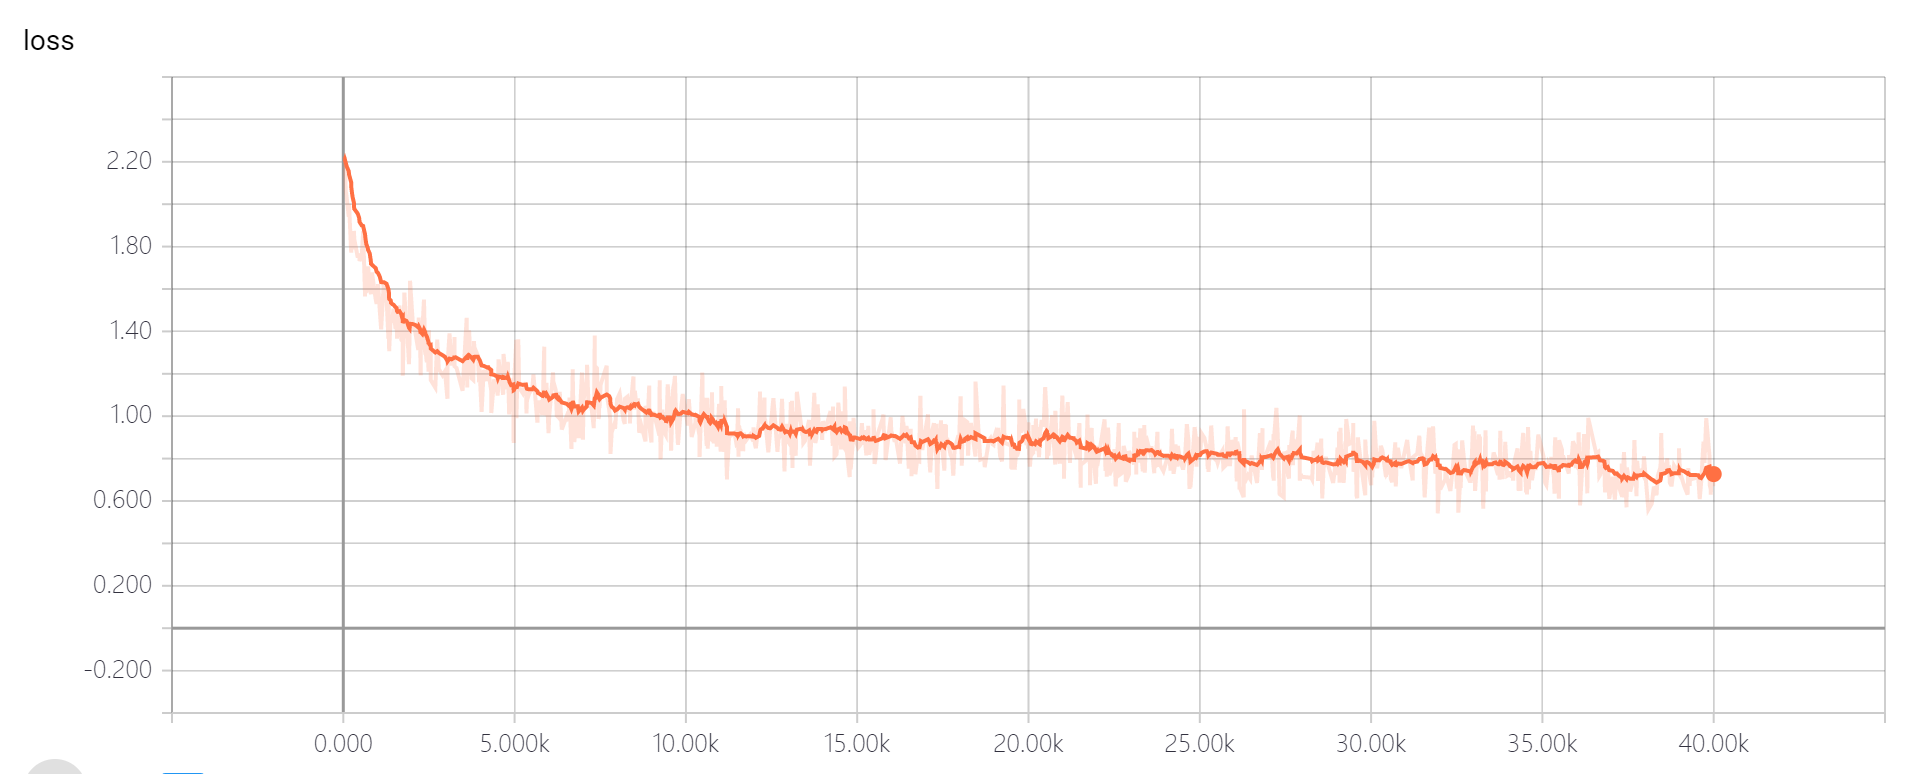
\includegraphics[width=440pt,height=170pt]{loss.png}
\caption{Training Loss}
\label{loss}
\end{figure}

\begin{figure}[htbp]
\centering
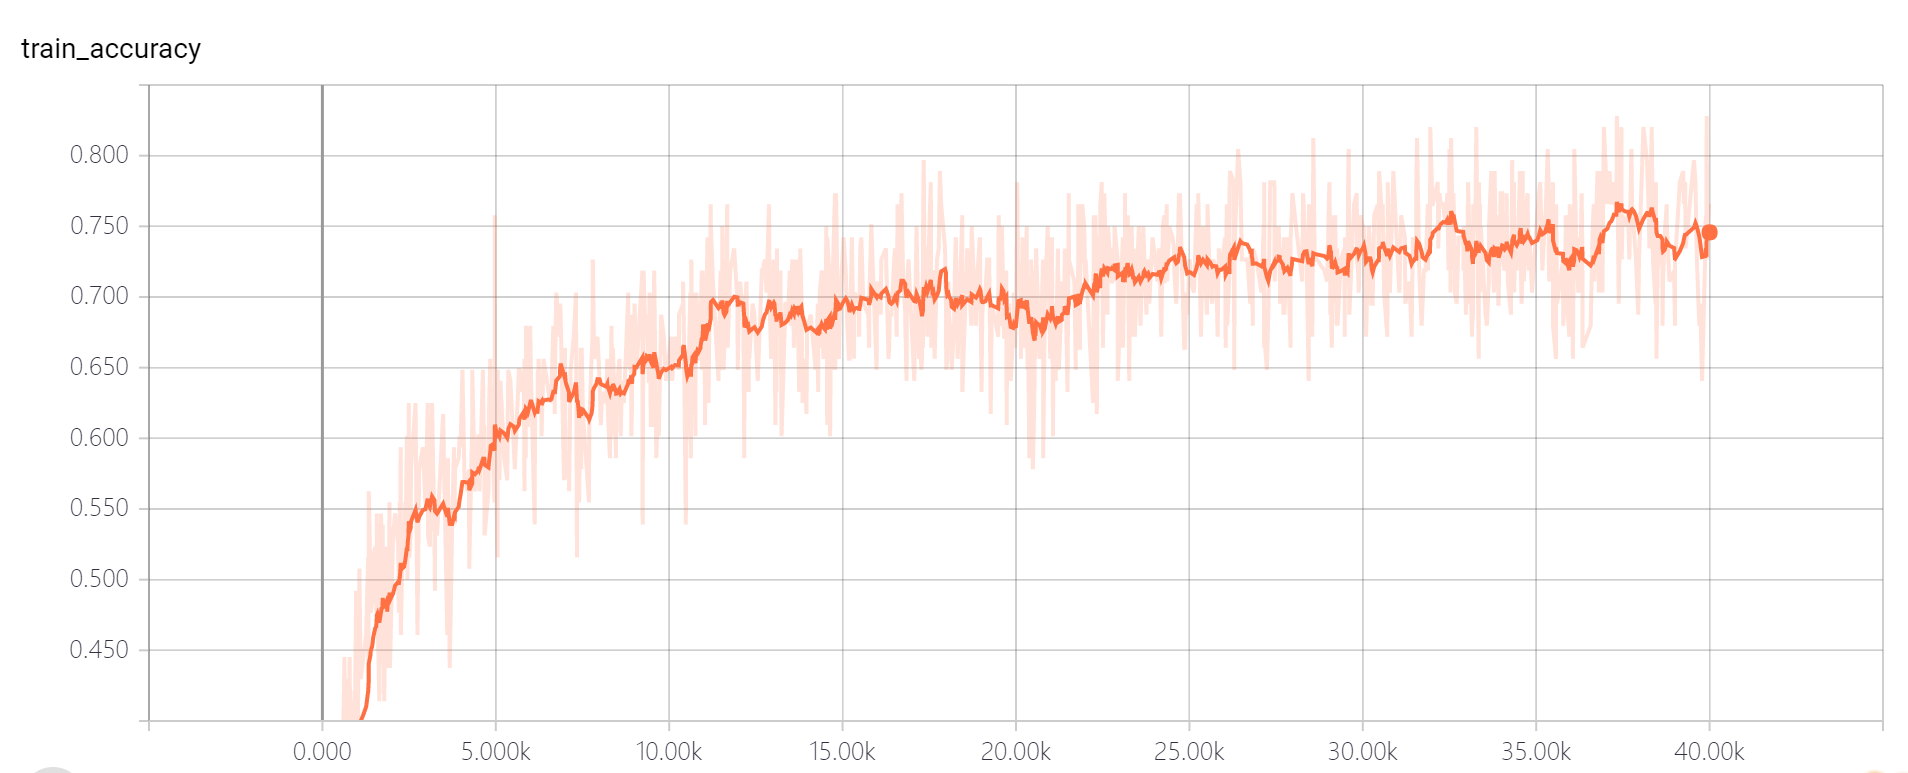
\includegraphics[width=440pt,height=170pt]{trainaccuracy.png}
\caption{Training Accuracy}
\label{accuracy}
\end{figure}

\begin{figure}[htbp]
\centering
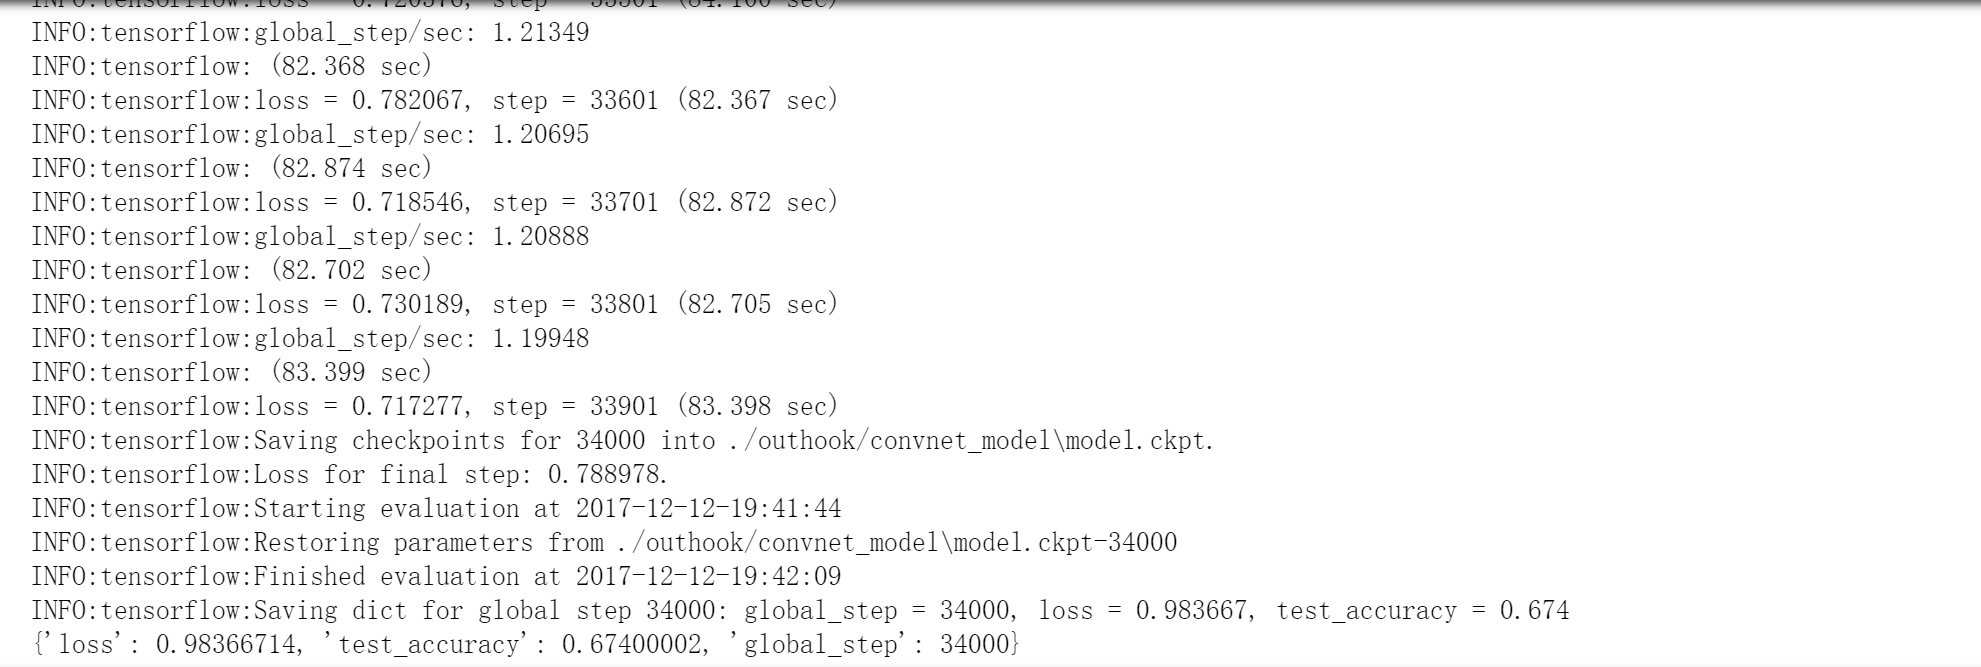
\includegraphics[width=440pt,height=150pt]{bestaccuracy.png}
\caption{Screen Shot}
\label{best}
\end{figure}
From the plot, we can see that the accuracy increased very slowly after 20k steps. The final training accuracy is about $75\%$, close to the final test accuracy $67.4\%$, indicates the model is not overfitting . \\
To further improve the test performance, we could add more layers or use some existed feature extraction process.

\section{Inception-V3 Model}
In this part, we use the similar strategy in hw4, but we cropped the image to $28\times 28$ then reshaped it to $299\times299$, recomputed the bottlenecks and got the final training accuracy after 2500 steps was about $90.2\%$, the test accuracy was about $81.5\%$. \\
The following graphs show the accuracy and cross entropy of the training step and a screen shot of the detailed value of train and test accuracy.
\begin{figure}[htbp]
\centering
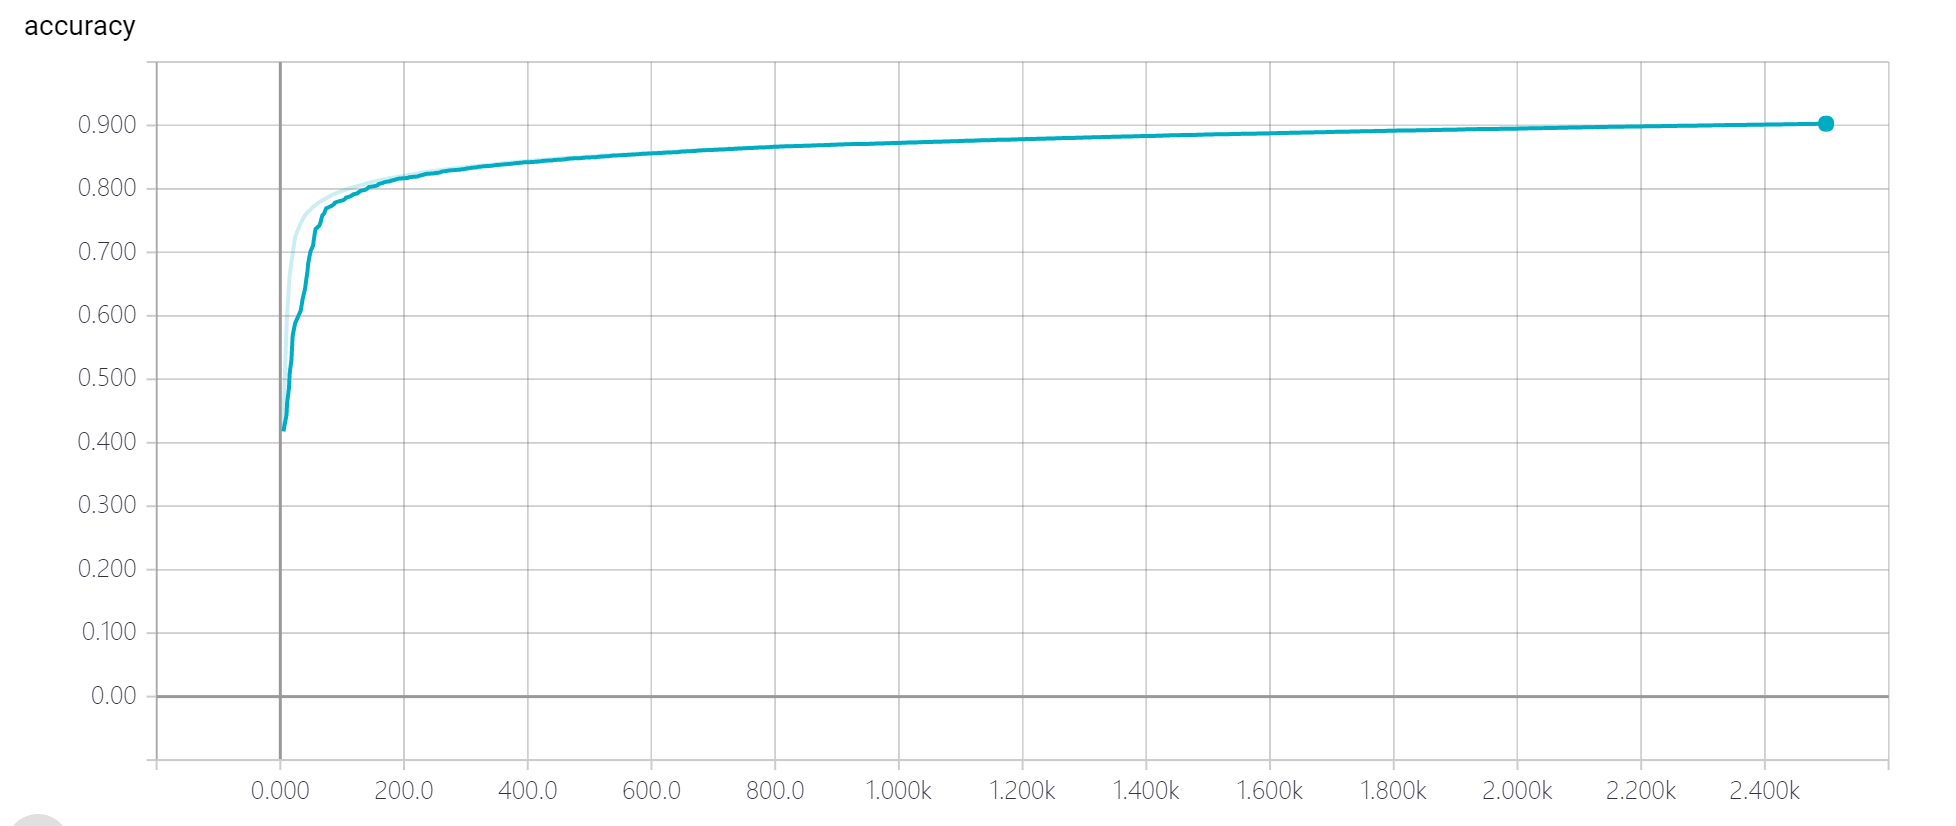
\includegraphics[width=440pt,height=150pt]{inceptionaccuracy.png}
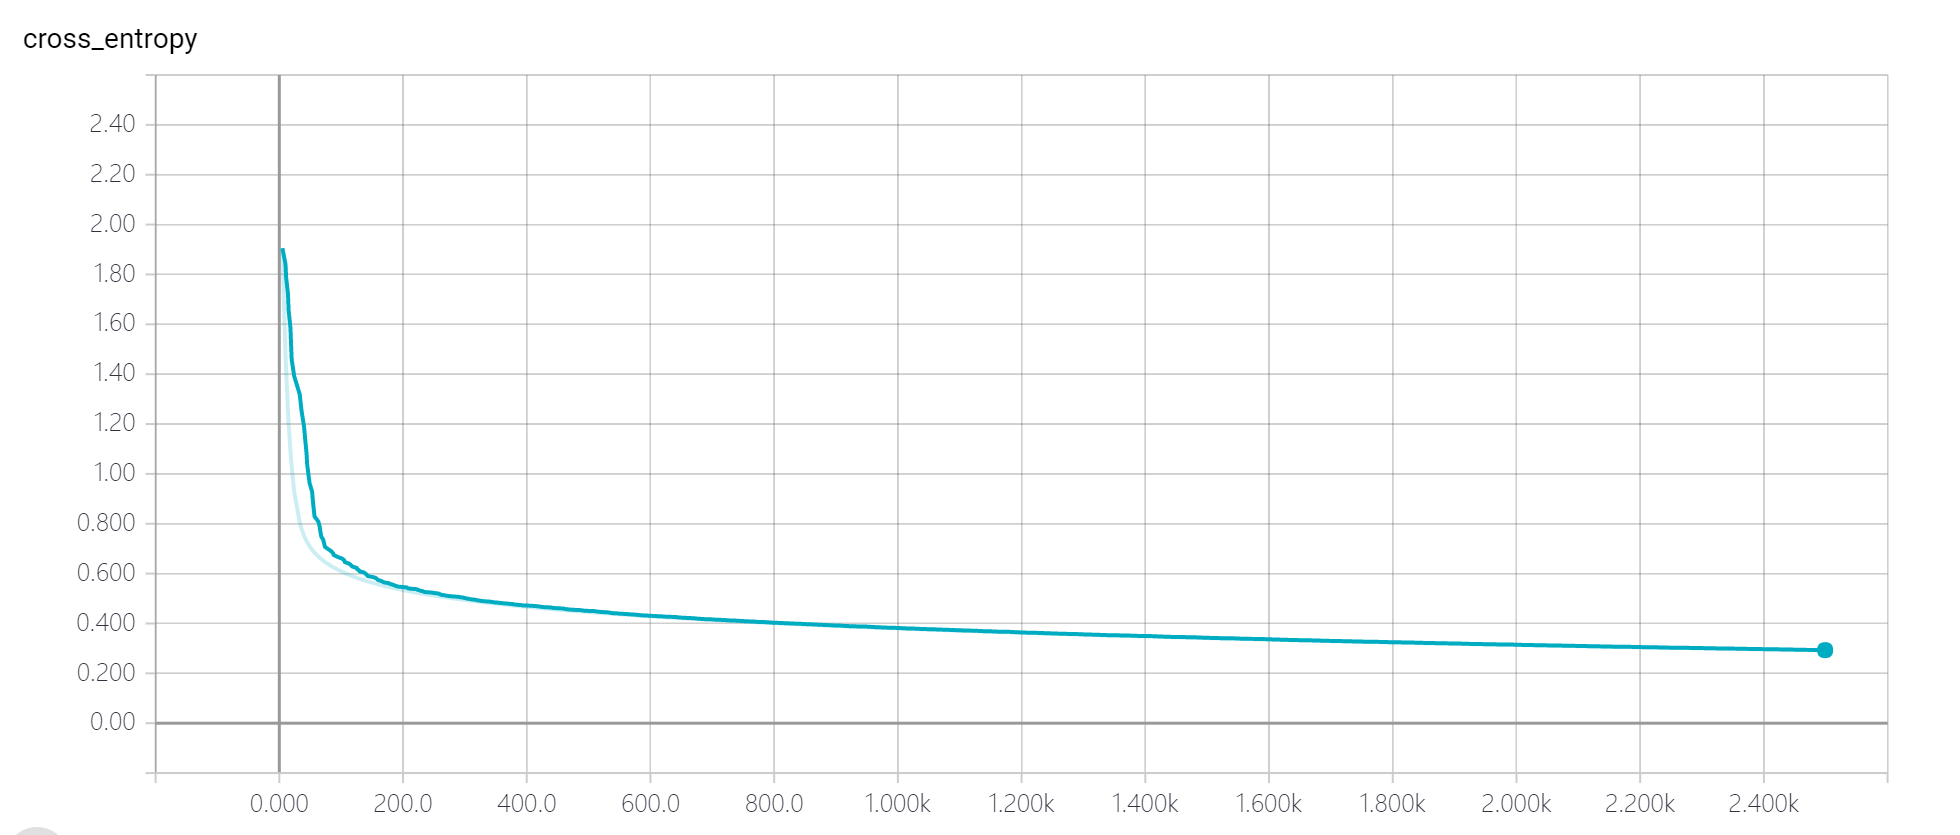
\includegraphics[width=440pt,height=150pt]{inceptioncross.png}
\caption{Inception-V3 ac and loss}
\label{in-ac}
\end{figure}

\begin{figure}[htbp]
\centering
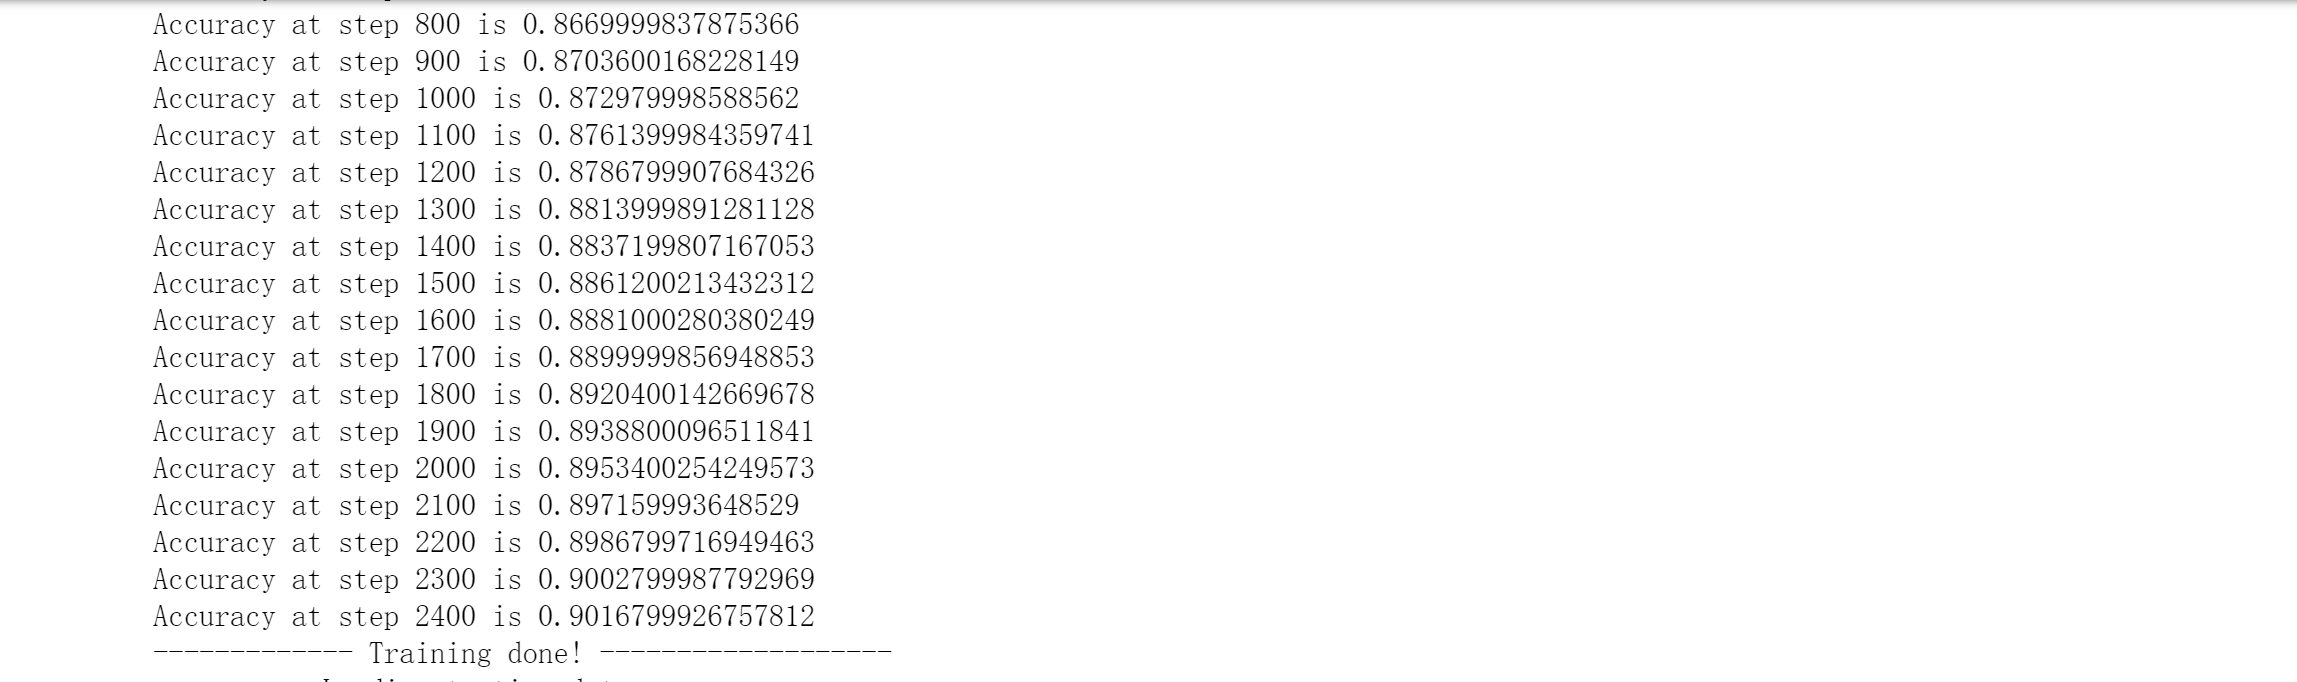
\includegraphics[height=180pt]{inceptiontrain.png}
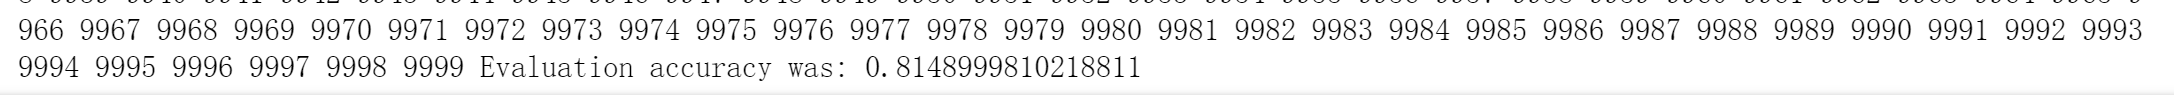
\includegraphics[width=480pt]{inceptiontest.png}
\caption{Inception-V3 training and test}
\label{in-train}
\end{figure}

\section{Conclusion}
We already showed two models we worked on for CIFAR-10 classification problem: CNN model and Inception-V3 model. As we can see from the result, Inception-V3 model, without overfitting problem, gives a higher accuracy on both training set and testing set than the 9-layer CNN model. \\
Indeed, the advanced magical way Inception-V3 model used to extract the features is the key to the good performance. So it is really important to pay attention to feature extraction process during the design of our own CNN.


\begin{thebibliography}{99}
\bibliographystyle{siam}
\setlength{\baselineskip}{14pt}
\bibitem{Xaiver}Glorot, Xavier and Bordes, Antoine and Bengio, Yoshua.
\newblock{\em Deep Sparse Rectifier Neural Networks}, Proceedings of the Fourteenth International Conference on Artificial Intelligence and Statistics, 2011, pp315-323.
\end{thebibliography}

\newpage

\begin{appendices}

\section{Python Code}
\begin{lstlisting}[language=Python]
Part 1: CNN model
# import the package we need
import numpy as np
import tensorflow as tf

def unpickle(file):
    '''Read the raw data, a dictionary which contains the features,
    labels and other information'''
    import pickle
    with open(file, 'rb') as fo:
        dict = pickle.load(fo, encoding='bytes')
    return dict

def get_train():
    '''Get all the 5 trainsets and convert the datatype Unit8 to float32
    Output:
        trdata: [50000, 3072] RGB features
        trlabels: [50000,] training labels from 0-9
    '''
    data = unpickle('./cifar-10-batches-py/data_batch_1')
    trdata = np.asarray(data[b'data'], dtype= np.float32)
    trlabels = np.asarray(data[b'labels'], dtype= np.float32)
    for i in range(2,6):
        data = unpickle('./cifar-10-batches-py/data_batch_{}'.format(i))
        trdata = np.row_stack((trdata, (np.asarray(data[b'data'], dtype= np.float32))))
        trlabels = np. concatenate((trlabels, (np.asarray(data[b'labels'],
                                    dtype= np.float32))), 0)
    return(trdata, trlabels)

def get_test():
    '''Get the testsets and convert the datatype Unit8 to float32
    Output:
        tedata: [10000, 3072] RGB features
        telabels: [10000,] test labels from 0-9
    '''
    data= unpickle('./cifar-10-batches-py/test_batch')
    tedata = np.asarray(data[b'data'], dtype= np.float32)
    telabels = np.asarray(data[b'labels'], dtype= np.float32)
    return(tedata, telabels)

# add the weight decay to avoid overfitting
def weight_decay_variable(name, shape, stddev, wd):
    dtype = tf.float32
    var = tf.get_variable(name, shape,
                        initializer=tf.truncated_normal_initializer(stddev=stddev),
                        dtype=dtype)
    # define the weight decay
    weight_decay = tf.multiply(tf.nn.l2_loss(var), wd, name='weight_loss')
    # add the weight to total loss
    tf.add_to_collection('losses', weight_decay)
    return var

crop_size = 28

# for training step, crop and distort the image
def preprocess_train_image(x):
    '''Input:
            x: a training data with size [1, 3072]
       Output:
           float_image: a distorted training data with size [1, 28x28x3]
    '''
    # Randomly crop the original image.
    distorted_image = tf.random_crop(x, [crop_size, crop_size, 3])

    # Randomly flip the original image horizontally.
    distorted_image = tf.image.random_flip_left_right(distorted_image)

    # Randomly distort the brightness of the image.
    distorted_image = tf.image.random_brightness(distorted_image, max_delta=1.0)

    # Randomly distort the contrast of the image.
    distorted_image = tf.image.random_contrast(distorted_image, lower=0.2, upper=1.0)

    # Subtract off the mean and divide by the variance of the pixels.
    float_image = tf.image.per_image_standardization(distorted_image)

    # Set the dimension of the output
    float_image.set_shape([crop_size, crop_size, 3])
    return (float_image)

# for testing step, only crop the image
def preprocess_test_image(x):
    '''Input:
            x: a testing data with size [1,32*32*3]
       Output:
           float_image: a croped data with size [1,28*28*3]
    '''
    # crop the center of the image
    resized_image = tf.image.resize_image_with_crop_or_pad(x, crop_size, crop_size)
    float_image = tf.image.per_image_standardization(resized_image)
    float_image.set_shape([crop_size, crop_size, 3])
    return(float_image)

def create_cnnmodel(features, labels, mode):
    """Build the CNN Model"""
    # Input layer
    input_features = tf.reshape(features["x"], [-1, 32, 32, 3])
    input_layer = tf.map_fn(preprocess_test_image, input_features)
    if mode == tf.estimator.ModeKeys.TRAIN:
        input_layer = tf.map_fn(preprocess_train_image, input_features)

    # Convolutional Layer #1 (output:[batch_size, 28, 28, 32])
    conv1 = tf.layers.conv2d(inputs=input_layer, filters=32, kernel_size=[5, 5],
                             padding="same", activation=tf.nn.relu, name="conv1")

    # Pooling Layer #1 (output:[batch_size, 14, 14, 32])
    pool1 = tf.layers.max_pooling2d(inputs=conv1, pool_size=[2, 2],
                                    strides=2, name="pool1")

    # Convolutional Layer #2 (output:[batch_size, 14, 14, 64])
    conv2 = tf.layers.conv2d(inputs=pool1, filters= 64, kernel_size=[5, 5],
                             padding="same", activation=tf.nn.relu, name="conv2")

    # Pooling Layer #2 (output:[batch_size, 7, 7, 64])
    pool2 = tf.layers.max_pooling2d(inputs=conv2, pool_size=[2, 2],
                                    strides=2, name="pool2")

    # Convolutional Layer #3 (output:[batch_size, 7, 7, 64])
    conv3= tf.layers.conv2d(inputs=pool2, filters= 64, kernel_size=[5, 5],
                            padding="same", activation=tf.nn.relu, name="conv3")

    # Convolutional Layer #4 (output:[batch_size, 7, 7, 32])
    conv4 = tf.layers.conv2d(inputs=conv3, filters= 32, kernel_size=[3, 3],
                             padding="same", activation=tf.nn.relu, name="conv4")

    # Pooling Layer #3 (output:[batch_size, 3, 3, 32])
    pool3 = tf.layers.max_pooling2d(inputs=conv4, pool_size=[3, 3],
                                    strides=2, name="pool3")

    # Fully-connected Layer #1 (output:[batch_size, 384])
    with tf.variable_scope('fc1') as scope:
        reshape = tf.reshape(pool3, shape=[-1, 3*3*32])
        dim = reshape.get_shape()[1].value
        weights = weight_decay_variable("weights_fc1", shape=[dim, 384],
                                        stddev=0.04, wd=0.001)
        biases = tf.get_variable("biases_fc1", shape=[384],
                                 initializer=tf.constant_initializer(0.1))
        fc1 = tf.nn.relu(tf.matmul(reshape, weights)+ biases, name=scope.name)

    # Fully-connected Layer #2 (output:[batch_size, 192])
    with tf.variable_scope("fc2") as scope:
        weights = weight_decay_variable("weights_fc2", shape=[384, 192],
                                        stddev=0.04, wd=0.01)
        biases = tf.get_variable("bias_fc2", shape=[192],
                                 initializer=tf.constant_initializer(0.1))
        fc2 = tf.nn.relu(tf.matmul(fc1, weights)+ biases, name=scope.name)

    # Logits Layer (output:[batch_size, 10])
    with tf.variable_scope("softmax_logits") as scope:
        weights = weight_decay_variable("weights_out", shape=[192, 10],
                                        stddev=1.0/192, wd=0.0)
        biases = tf.get_variable("biases_out", shape=[10])
        logits = tf.add(tf.matmul(fc2, weights), biases, name=scope.name)

    # Prediction dictionary: pred_class is the prediction labels, from 0 to 9.
    predictions = {
        "pred_class": tf.argmax(logits, axis=1, name= "pred_class"),
        "probabilities": tf.nn.softmax(logits, name="softmax_tensor")
    }

    if mode == tf.estimator.ModeKeys.PREDICT:
        return tf.estimator.EstimatorSpec(mode=mode, predictions=predictions)

    # Calculate cross entropy and the total losses of each batch (for training steps)
    # change the labels into one_hot type, depth=10 means 10 labels
    onehot_labels = tf.one_hot(indices=tf.cast(labels, tf.int32), depth=10)
    # compute the cross entropy between the logits and true labels
    cross_entropy = tf.nn.softmax_cross_entropy_with_logits(labels = onehot_labels,
                                                            logits= logits)
    # compute the cross entropy loss
    cross_entropy_loss = tf.reduce_mean(cross_entropy, name='cross_entropy_loss')
    tf.add_to_collection('losses', cross_entropy_loss)
    # total loss is the cross entropy loss and the weight decay loss
    loss = tf.add_n(tf.get_collection('losses'), name='total_loss')
    # compute the training accuracy for visualization in the tensorboard
    labels_int = tf.cast(labels, tf.int64)
    accuracy = tf.reduce_mean(tf.cast(tf.equal(predictions["pred_class"],
                                               labels_int), tf.float32))

    # Construct the training optimizer
    if mode == tf.estimator.ModeKeys.TRAIN:
        # using Adamoptimizer and the learning rate = 0.001
        global_step= tf.train.get_global_step()
        optimizer = tf.train.AdamOptimizer(learning_rate=0.001)
        train_op = optimizer.minimize( loss=loss, global_step=tf.train.get_global_step())

        # Create the summary graph for loss, logits and training accuracy
        #cd C:\Users\qn_li\Columbia\Advanced Machine Learning\Project
        #tensorboard --logdir=./outhook/tb
        tf.summary.scalar("loss", loss)
        tf.summary.histogram('logits', logits)
        tf.summary.scalar('train_accuracy', accuracy)
        summary_hook = tf.train.SummarySaverHook(save_steps=1, output_dir='./outhook/tb',
                                                 summary_op=tf.summary.merge_all())

        return tf.estimator.EstimatorSpec(mode=mode, loss=loss, train_op=train_op, training_hooks=[summary_hook])

    # Compute the test accuracy and construct the evaluate optimizer
    eval_metric_ops = { "test_accuracy": tf.metrics.accuracy(labels=labels, predictions=predictions["pred_class"])}

    return tf.estimator.EstimatorSpec(
        mode=mode, loss=loss, eval_metric_ops=eval_metric_ops)

def main():
    # Load training and eval data and convert the datatype from Unit8 to float32
    train_data, train_labels = get_train()
    eval_data, eval_labels = get_test()

    # Create the Estimator
    cifar10_classifier = tf.estimator.Estimator(model_fn= create_cnnmodel, model_dir="./outhook/convnet_model")

    # Set up logging for predictions
    #tensors_to_log = {"probabilities": "softmax_tensor"}
    tensors_to_log={}
    logging_hook = tf.train.LoggingTensorHook(tensors=tensors_to_log, every_n_iter=100)

    # Train the model
    train_input_fn = tf.estimator.inputs.numpy_input_fn(
                            x={"x": train_data}, y=train_labels,                                                        batch_size= 128, num_epochs=100, shuffle=True)

    train_results = cifar10_classifier.train( input_fn=train_input_fn, steps= total_steps, hooks=[logging_hook])

    # Evaluate the model and print results
    eval_input_fn = tf.estimator.inputs.numpy_input_fn(x={"x": eval_data},
                                                       y=eval_labels,
                                                       num_epochs=1, shuffle=False)

    eval_results = cifar10_classifier.evaluate(input_fn=eval_input_fn)
    print(eval_results)

total_steps = 38000
main()

Part 2: Inception_V3 model
import tensorflow as tf
import numpy as np
import os
os.environ['TF_CPP_MIN_LOG_LEVEL']='2'
import os.path
import transfer_learning_project as transfer_learning
import matplotlib.pyplot as plt
import scipy.misc
import glob
import sys
import random

# Ensure target log dir exists
INCEPTION_LOG_DIR = './tmp/inception_v3_log'
if not os.path.exists(INCEPTION_LOG_DIR):
    os.makedirs(INCEPTION_LOG_DIR)

# import traing and test data
training_images, _, label_maps = transfer_learning.create_image_lists(
    './cifar-10/train', testing_percentage=0, max_number_images=5001)

testing_images, _, _ = transfer_learning.create_image_lists(
    './cifar-10/test', testing_percentage=0, max_number_images=1001)

# check the length of the training_images and testing_images
print(len(training_images))
print(len(testing_images))

# Create the inception model.
graph, bottleneck, resized_input, softmax = transfer_learning.create_model()

# Use a summary writer to write the loaded model graph and display it in tensorboard.
# tensorboard --logdir=./tmp/inception_v3_log
with graph.as_default():
    jpeg_data, decoded_image = transfer_learning.make_jpeg_decoding()
    # Define summaries for tensorboard
    # create hsitogram summary for output softmax and bottleneck
    tf.summary.histogram('output', softmax)
    tf.summary.histogram('bottleneck', bottleneck)
    # create summary for input image
    tf.summary.image('input', resized_input)
    summary_op = tf.summary.merge_all()

    with tf.Session() as sess:
        summary_writer = tf.summary.FileWriter(INCEPTION_LOG_DIR, sess.graph)
        sess.run(tf.global_variables_initializer())

def classify_image(session, image_path, summary_op):
    """This functions reads a single image from disk and classifies
    the image using the pre-trained network.

    Parameters
    ----------
    session: the tensorflow session to use to run the operation
    image_path: a string corresponding to the path of the image to load
    summary_op: the summary operation.

    Returns
    -------
    label: an integer representing the label of the classified example.
    softmax_output: the network's output multinomial probabilities
    """
    # Open single image file and extract data
    with open(image_path, 'rb') as f:
        image_data = f.read()
    # run the train step and add the summary to tensorboard
    input_value = session.run((decoded_image), {jpeg_data: image_data})
    softmax_output = session.run(softmax, feed_dict={resized_input: input_value})
    summary = session.run(summary_op, {jpeg_data: image_data, resized_input: input_value})
    summary_writer = tf.summary.FileWriter(INCEPTION_LOG_DIR, session.graph)
    summary_writer.add_summary(summary)
    # Return label
    return(np.argmax(softmax_output),softmax_output)

def compute_bottleneck(session, image_data):
    """Computes the bottleneck for a given image

    Parameters
    ----------
    session: the tensorflow session to use for the computation.
    jpeg_data_tensor: the tensor to feed the jpeg data into.
    bottleneck_tensor: the tensor representing.
    image_data: a byte sequence representing the encoded jpeg data.

    Returns
    -------
    A numpy array containing the bottleneck information for the image.
    """
    new_value = session.run(decoded_image, feed_dict= {jpeg_data: image_data})
    bottleneck_values = session.run(bottleneck, feed_dict= {resized_input: new_value})
    return(bottleneck_values)

# This cell generates all the bottlenecks and it will take a
# long time since there are 50000 bottlenecks should be computed.
with graph.as_default():
    with tf.Session() as session:
        transfer_learning.cache_bottlenecks(compute_bottleneck, session, training_images)

# This loads the training data as a matrix of training examples
# and a vector of labels
training_data_set = transfer_learning.create_training_dataset(training_images)

def make_final_layers(bottleneck_tensor, num_classes):
    """Create the operations for the last layer of the network to be retrained.
    Parameters
    ----------
    bottleneck_tensor: the bottleneck tensor in the original network
    num_classes: the number of output classes

    Returns
    -------
    bottleneck_input: the input placeholder for the bottleneck values
    label_input: the input placeholder for the label values
    logits: the tensor representing the unnormalized log probabilities
        for each class.
    train_step: an operation representing one gradient descent step.
    """
    bottleneck_tensor_size = int(bottleneck.shape[1])

    with tf.variable_scope('input'):
        # This is the input for the bottleneck. It is created
        # as a placeholder with default. During training, we will
        # be passing in the bottlenecks, but during evaluation,
        # the value will be propagated from the bottleneck computed
        # from the image using the full network.
        bottleneck_input = tf.placeholder_with_default(
            bottleneck_tensor,
            [None, bottleneck_tensor_size],
            'bottleneck_input')

        # This is the input for the label (integer, 1 to number of classes)
        label_input = tf.placeholder(tf.int64, [None], name='label_input')

    # Define weights, biases, and logit transforms
    logits = tf.layers.dense(bottleneck_input, num_classes)
    # Compute the cross entropy loss
    loss = tf.losses.sparse_softmax_cross_entropy(labels=label_input, logits=logits)
    # Create a summary for the loss
    loss_summary = tf.summary.scalar('cross_entropy', loss)
    # Create a Gradient Descent Optimizer
    # optimizer = tf.train.GradientDescentOptimizer(0.1)
    optimizer = tf.train.AdamOptimizer(learning_rate=0.001)
    # Obtain a function which performs a single training step
    train_step = optimizer.minimize(loss)
    return bottleneck_input, label_input, logits, train_step, loss_summary

def compute_accuracy(labels, logits):
    """Compute the accuracy for the predicted output.

    Parameters
    ----------
    labels: The input labels (in a one-hot encoded fashion).
    predicted_output: The predicted class probability for each output.

    Returns
    -------
    A tensor representing the accuracy.
    """
    prediction = tf.argmax(logits, 1, name='pred_class')
    accuracy = tf.reduce_mean(tf.cast(tf.equal(prediction, labels), tf.float32))
    accuracy_summary = tf.summary.scalar('accuracy', accuracy)

    return accuracy, accuracy_summary

# We create the necessary operations to fine tune the model.

with graph.as_default():
    bottleneck_input, label_input, logits, train_step, loss_summary = make_final_layers(bottleneck, len(label_maps))
    accuracy, accuracy_summary = compute_accuracy(label_input, logits)
    summary_op = tf.summary.merge([loss_summary, accuracy_summary])

def execute_train_step(session: tf.Session, summary_writer: tf.summary.FileWriter, current_step: int):
    """This function runs a single training step.

    You may wish to print some progress information as you go along.

    Parameters
    ----------
    session: the tensorflow session to use to run the training step.
    summary_writer: the summary file writer to write your summaries to.
    current_step: the current step count (starting from zero)
    """
    _, ac, summary = session.run((train_step, accuracy, summary_op),
                       feed_dict={bottleneck_input: training_data_set['bottlenecks'],
                                  label_input: training_data_set['labels']
                                 })

    summary_writer.add_summary(summary, current_step)

    if current_step % 100 == 0:
        print('Accuracy at step {0} is {1}'.format(current_step, ac))


def evaluate_images(session: tf.Session, images_jpeg_data: [bytes], labels: [int]):
    """This function will evaluate the accuracy of our model on the specified data.

    Parameters
    ----------
    session: the tensorflow session to use to run the evaluation step.
    images_jpeg_data: a list of strings, with each element in the list corresponding
        to the jpeg-encoded data for a given image
    labels: a list of integers, with each element in the list corresponding to the label
        of a given image.

    Returns
    -------
    This function should return the accuracy as a floating point number between
    0 and 1 (proportion of correctly classified instances).
    """
    correct = []
    i = 0
    for label, jpeg in zip(labels, images_jpeg_data):
        image_data = session.run(decoded_image, feed_dict={jpeg_data: jpeg})
        ac = session.run(accuracy, feed_dict={resized_input: image_data, label_input: [label]})
        correct.append(ac)
        print(i,end=" ")
        i+=1

    return np.mean(correct)

# run the training and evaluation!
with graph.as_default():
    with tf.Session() as session:
        print('------------- Starting training ----------------')
        session.run(tf.global_variables_initializer())
        summary_writer = tf.summary.FileWriter(os.path.join(INCEPTION_LOG_DIR, 'retrained'), graph)
        for i in range(2500):
            execute_train_step(session, summary_writer, i)
        summary_writer.close()
        print('------------- Training done! -------------------')
        print('---------- Loading testing data ----------------')
        tlabels, timages = transfer_learning.get_testing_data(testing_images)
        print('----------- Evaluating on testing --------------')

        eval_accuracy = evaluate_images(session, timages, tlabels)
        print('Evaluation accuracy was: {0}'.format(eval_accuracy))


\end{lstlisting}

\end{appendices}
%%%%%%%%%%%%%%%%%%%%%%%%%%%%%%End%%%%%%%%%%%%%%%%%%%%%%%%%%%%%%%%
\end{document}

